\documentclass[12pt]{beamer}

\def\languages{french, english}

%%%%%%%%%%%%%%%%%%% Theme

\usetheme{metropolis}

%%%%%%%%%%%%%%%%%%% Libraries

%%%%%%%%%% Packages

\usepackage[
backend=biber,
style=numeric-comp,
sorting=none,
maxbibnames=99
]{biblatex}
%%%%%%%%%% Packages

%%%%% Coding tools

\usepackage{comment}
\usepackage{xstring}

%%%%% Encoding

\usepackage[utf8]{inputenc}
\usepackage[T1]{fontenc}
\usepackage{eurosym}

%%%%% Languages

\ifx\languages\undefined
	\usepackage[english]{babel}
\else
	\usepackage[\languages]{babel}
\fi

\def\languagefile{./include/languages/\languagename.tex}
\InputIfFileExists{\languagefile}{}

%%%%% Style

\usepackage{csquotes}
\usepackage{color}
\usepackage{textpos}

\newcommand\titlelogo[1]{
	\titlegraphic{
		\hfill\includegraphics[height=0.2\textheight]{#1}
	}
}

\newcommand\framelogo[1]{
	\addtobeamertemplate{frametitle}{}{
		\begin{textblock*}{\textwidth}(\textwidth,-1.28\baselineskip)
			\includegraphics[height=\baselineskip]{#1}
		\end{textblock*}
	}
}

%%%%%%%%%% Packages

\usepackage{float}
\usepackage[skip=1em]{caption}

\usepackage{array}
\usepackage{multirow}
\usepackage{multicol}

%%%%%%%%%% Features

%%%%% Settings

\renewcommand{\arraystretch}{1.2}

%%%%% Commands

\newcommand\noskipcaption[1]{\caption{#1}\vspace{-1em}}
\newcommand\noskipcaptionstar[1]{\caption*{#1}\vspace{-1em}}

%%%%%%%%%% Packages

\usepackage{siunitx}

%%%%%%%%%% Features

%%%%% Settings

\ifx\decimalsign\undefined
\else
    \sisetup{output-decimal-marker = \decimalsign}
\fi


%%%%%%%%%%%%%%%%%%% Bibliography

\addbibresource{resources/bib/sample.bib}

%%%%%%%%%%%%%%%%%%% Titlepage

\title{Renewable Energy Production Forecast}
\subtitle{PROJ0016 - Big Data Project}
\author{Yann Claes, Gaspard Lambrechts and François Rozet}
\institute{University of Liège}
\date{\today}
\titlelogo{resources/pdf/logo.pdf}
\framelogo{resources/pdf/logo.pdf}

%%%%%%%%%%%%%%%%%%%

\begin{document}

\maketitle

\section{Scope of the project}

\begin{frame}{Structure}
    The project is divided in two independent parts:
    \begin{itemize}
        \item \alert{Production models} : predicting the production from the characteristics of a production unit and the weather at the unit location;
        \item \alert{Identification of production units} : for the considered area (Liège), extracting all renewable energy production units and their characteristics.
    \end{itemize}
    \visible<2->{Then, by combining the two parts, we can estimate the production of renewable at Liège tomorrow.}
\end{frame}

\begin{frame}{Production models}
    \alert{Initially}, we could use theoretical models to predict power production.
    \begin{itemize}
        \item<1-> Power curve of wind turbines;
        \only<1>{
        \vspace{0.5em}
        \begin{figure}
            \centering
            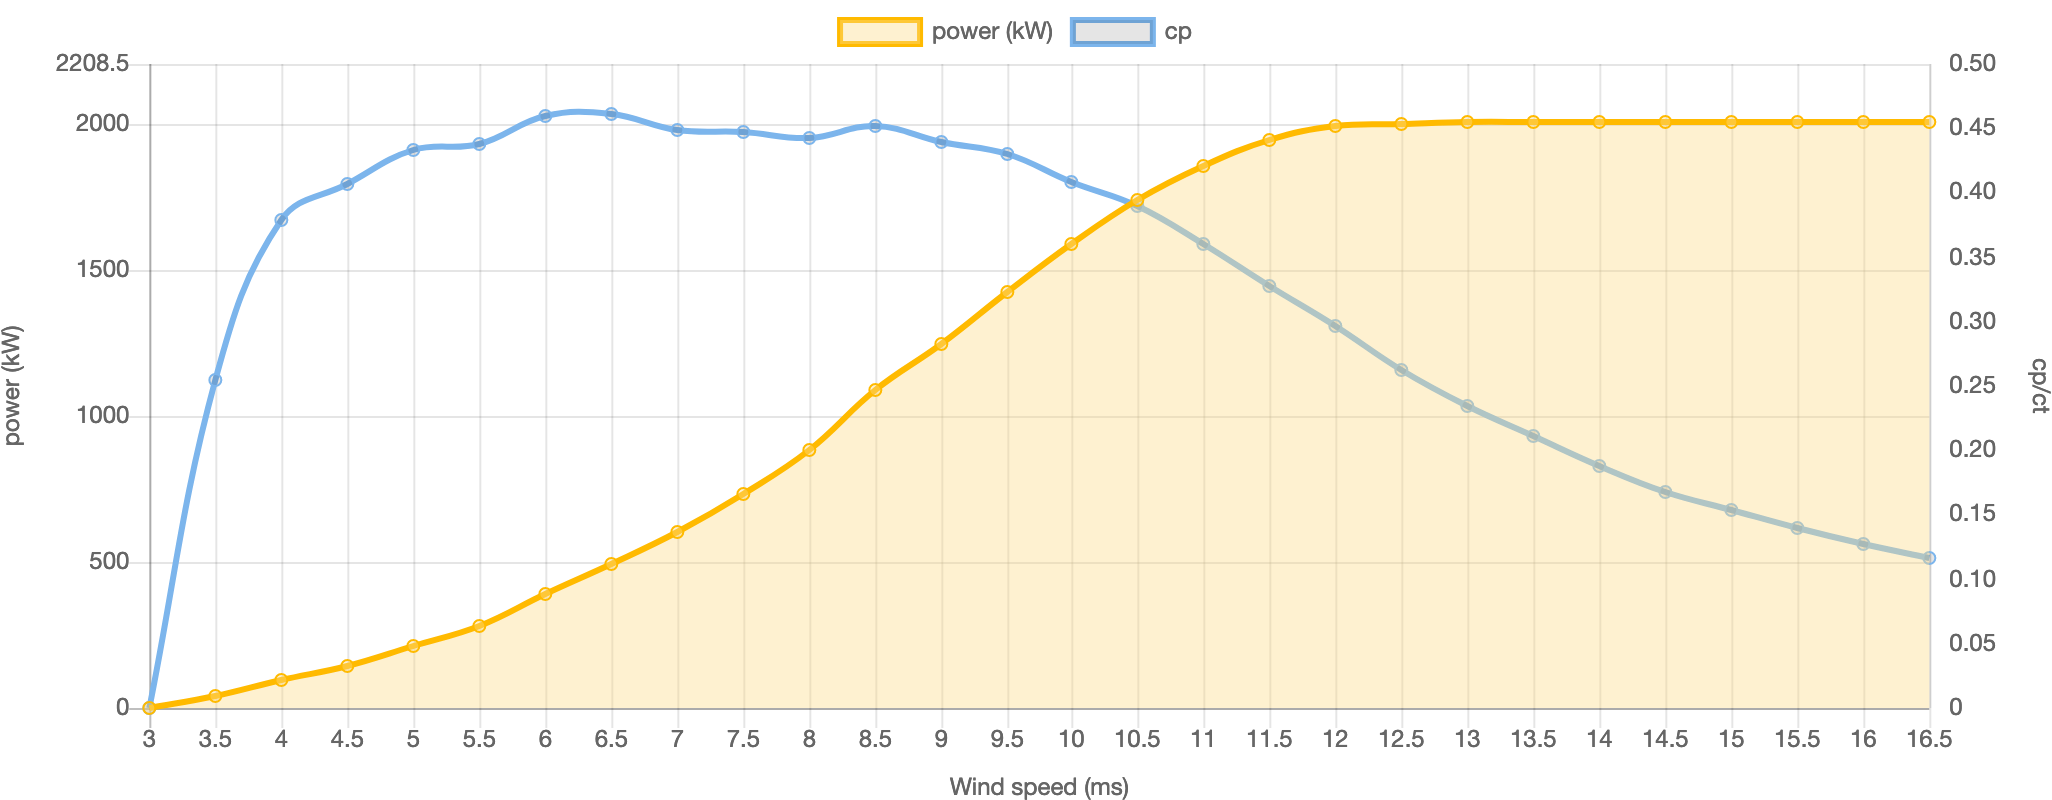
\includegraphics[width=0.9\textwidth]{resources/power_curve.png}
            \caption*{Example of power curve for Vega V90 wind turbine}
        \end{figure}
        }
        \item<2-> Production model of photovoltaic panels with respect to the irradiance, temperature and orientation.
        \only<2>{$$ Power = f(radiation, orientation, tilt, efficiency) $$}
    \end{itemize}
\end{frame}

\begin{frame}{Production units}
    For wind power, each power plant is identified by \alert{Elia}. For PV, the \alert{CWaPE} maintains a database of installed power for each municipality. \visible<2->{\alert{But},
    \begin{itemize}
        \item Data from \alert{CWaPE} is two years old and gives no information on the location, orientation, tilt or model/type for each PV unit.
        \item We don't want our forecast to be dependent on the availability of data on PV units.
    \end{itemize}
    }
\end{frame}

\begin{frame}{Production units}
    Thus, it has been chosen to try using \alert{satellite imagery}. The strength of this approach is that it is not restricted to any area or scale.
    \begin{figure}
        \centering
        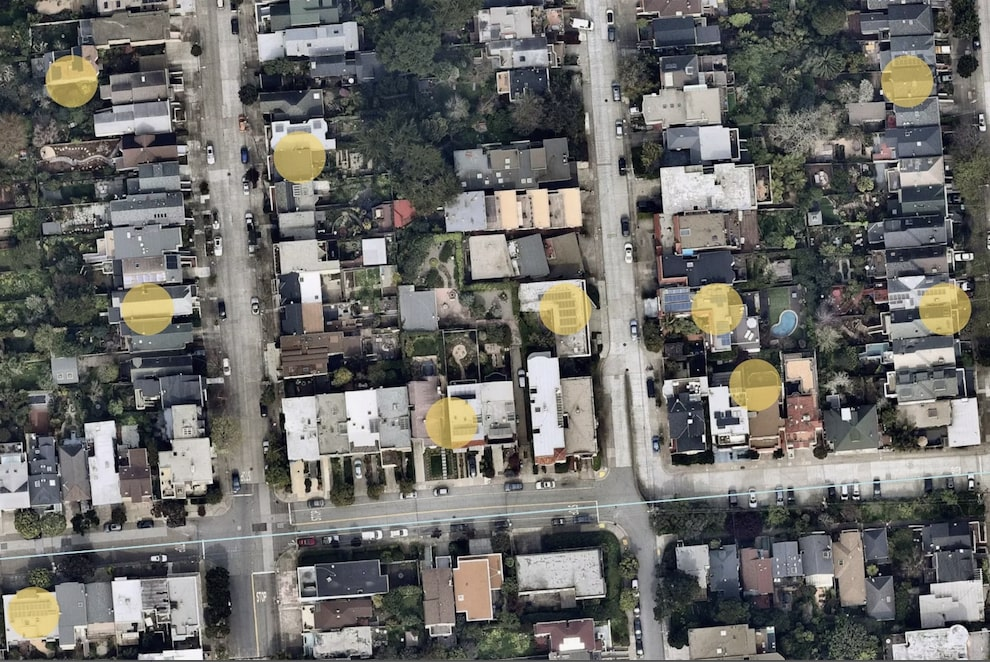
\includegraphics[width=0.6\textwidth]{resources/satellite.jpg}
        \caption*{Recognition of PV on satellite image using \alert{DeepSolar} software. \cite{deepsolar}}
    \end{figure}
\end{frame}

\begin{frame}{Global production forecast}
    By combining the production models and production units data, we could predict the global renewable energy production in Liège, but also in Walloonia and Belgium with respect to the \alert{weather forecast}.
    \visible<2->{$$model + units + weather \, forecast = production \, forecast$$}
    
\end{frame}
\begin{frame}{Global production forecast}
    To assess the quality of our predictions, we will compare our model with the production data from \alert{Elia}/\alert{APERe}\footnotemark[1].

    \footnotetext[1]{The production measures of \alert{Elia} and \alert{APERe} probably don’t take into account the electrical production which is not re-injected in the network for PV.}
\end{frame}

\section{Models}

\begin{frame}{Photovoltaic panels production}
    \begin{itemize}
        \item Theoretical model(s);
        \item \texttt{pvlib} Python library \cite{pvlib};
        \item ...
    \end{itemize}
\end{frame}

\begin{frame}{Wind farms production}
    \begin{itemize}
        \item Using the theoretical model;
        \item ...
    \end{itemize}
\end{frame}

\begin{frame}{Photovoltaic panels units}
    \begin{itemize}
        \item Deep learning and computer vision from satellite imagery;
        \item \alert{DeepSolar} GitHub repository \cite{deepsolar};
        \item ...
    \end{itemize}
\end{frame}

\begin{frame}{Wind farms units}
    \begin{itemize}
        \item Data from electricity provider(s);
        \item ...
    \end{itemize}
\end{frame}

\section{Data}

\begin{frame}{Weather data}
    \begin{itemize}
        \item Solar flow, temperatures and forecast (two locations) from the \alert{Laboratoire de Climatologie} of ULiège;
        \item Weather data from the \alert{Thermodynamics Laboratory} from the Aerospace and Mechanical Engineering Department of ULiège;
        \item Public API’s \alert{OpenWeatherMap} \cite{openweathermap}.
    \end{itemize}
\end{frame}

\begin{frame}{Photovoltaic panels data}
    \begin{itemize}
        \item Production of the photovoltaic panels of the \alert{Grands Amphitéatres’ parkings} (MySQL access to real time and past data).
        \item Number of photovoltaic panels and installed power per municipality provided by \alert{CWaPE} \cite{cwape}.
    \end{itemize}
\end{frame}

\begin{frame}{Wind farms data}
    \begin{itemize}
        \item All recorded wind farms from \alert{Elia} \cite{elia_wind}.
        \item Data from each electricity supplier having wind turbines also provided by \alert{CWaPE}.
    \end{itemize}
\end{frame}

\begin{frame}
    \printbibliography
\end{frame}

\end{document}
